\documentclass[tikz,border=10pt]{standalone}
\begin{document}
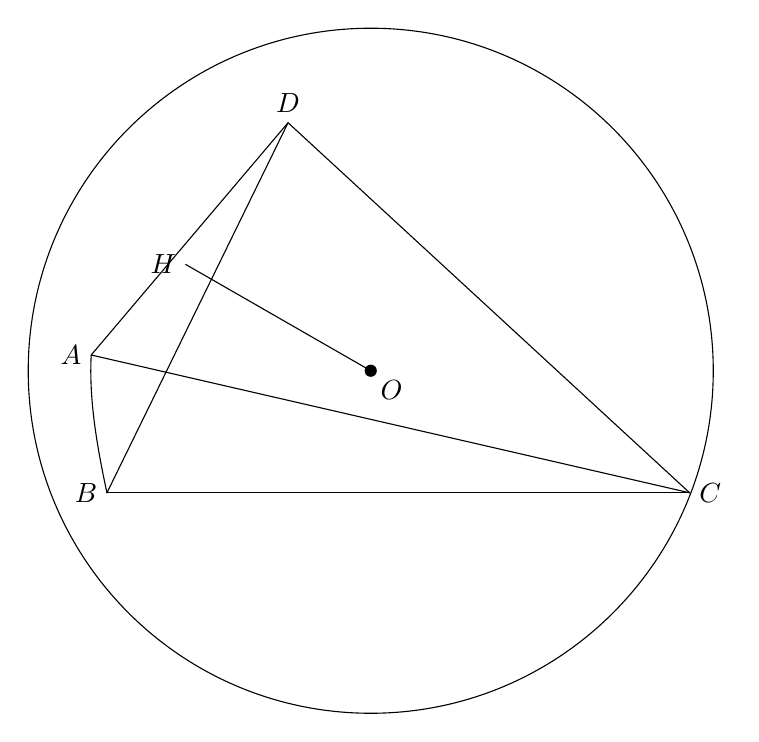
\begin{tikzpicture}[line cap=round,line join=round,scale=1]

% Points
\coordinate (O) at (0,0);
\coordinate (A) at (-3.55,0.20);
\coordinate (B) at (-3.35,-1.55);
\coordinate (C) at (4.05,-1.55);
\coordinate (D) at (-1.05,3.15);
\coordinate (H) at (-2.35,1.35);

% Circle
\draw (O) circle (4.35);

% Chords and segments
\draw (A) -- (D);
\draw (B) -- (D);
\draw (D) -- (C);
\draw (B) -- (C);
\draw (A) -- (C);
\draw (H) -- (O);

% Small arc-like inner curve near A and B
\draw (A) .. controls (-3.58,-0.35) and (-3.48,-0.95) .. (B);

% Point O
\fill (O) circle (2.2pt);

% Labels
\node[left] at (A) {$A$};
\node[left] at (B) {$B$};
\node[right] at (C) {$C$};
\node[above] at (D) {$D$};
\node[left] at (H) {$H$};
\node[below right] at (O) {$O$};

\end{tikzpicture}
\end{document}
